\chapter{XLore系统与应用接口构建}
\label{cha:xlore}

\section{本章引论}

跨语言知识库对全球知识的共享有着很大贡献。然而,中英文的跨语言知识库却很少,主要有以下几点原因:1)相对于丰富的英文知识,中文知识极度匮乏2)现有中英文跨语言对应关系的缺乏 3)本体语义分类树中,上下位关系存在错误。 为解决以上问题,我们在本章提出了一个构建中英文跨语言知识库(Cross-lingual knowledge base)的方法与流程,并将该知识库命名为{\heiti XLore}。具体来说,XLore囊括了英文维基,中文维基,百度百科与互动百科,四个在线百科的知识,以此来均衡中英文知识数量,同时,利用一个跨语言链接发现方法扩充跨语言链接集合,并引入了一个上下位关系判断,对分类树进行剪枝。详细流程见\ref{sec5:cross-lingual-knowledge-base}

当前一些知名的知识库将自己的数据展示或发布出来,DBpedia\footnote{http://wiki.dbpedia.org/}提供最新的数据集下载、数据统计记录,甚至开源代码;Probase\footnote{http://probase.msra.cn/Dataset.aspx}给出语义关系的数据集供研究人员使用,如is-a关系,同义词等。

然而中文知识库领域,搜狗、百度等商业化知识图谱仅供自家公司商用,并没有开放数据。Zhishi.me\footnote{http://zhishi.me/}作为第一个科研领域的中文知识库,早期提供实体查询接口与SPARQL查询接口,现数据与网站都久未更新。

我们的中英文跨语言知识库XLore,提供了数据展示页面、知识搜索功能、SPARQL查询接口、实例关系可视化、实体链接等多项功能,本章将具体阐述XLore网站系统的搭建(详见\ref{sec5:system-discribe})与实体链接接口的构建(详见\ref{sec5:entity-linking-api})。

\section{大规模中英文跨语言知识库XLore的构建}
\label{sec5:cross-lingual-knowledge-base}

XLore知识库融合中英文维基百科、百度百科与互动百科的信息,大大增加了中文知识数量,并利用大量跨语言链接提高中英文的融合度。构建过程中,我们首先从维基的数据存储文件,与百度、互动百科的网页信息中抽取出结构化语义信息,利用对齐关系合并成一体,并对分类体系进行剪枝,最后将数据转换成RDF三元组格式,导入Virtuoso数据库。具体流程图见图\ref{fig:xlore-preprocess}

\begin{figure}[H] 
  \centering
  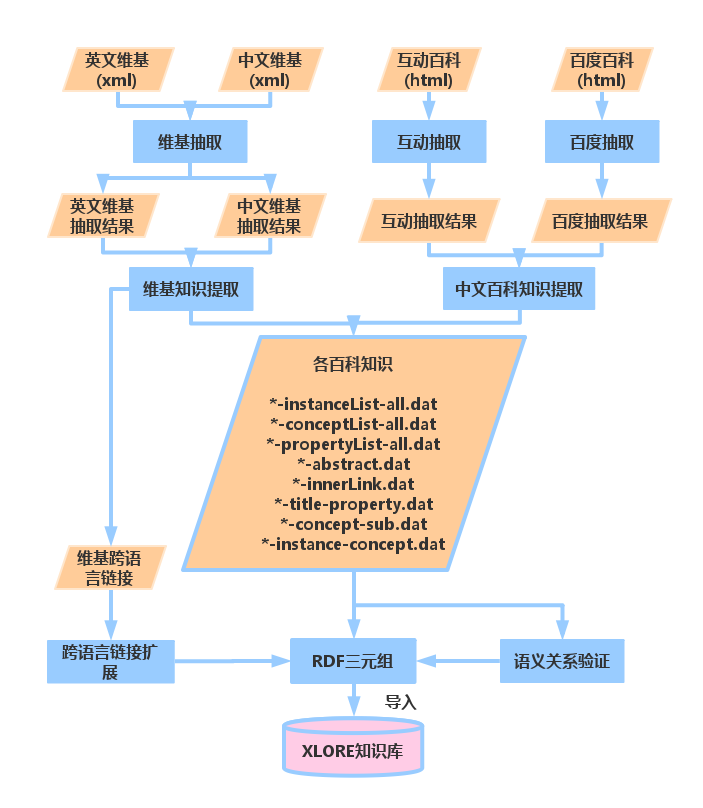
\includegraphics[width=0.8\columnwidth]{xlore_preprocess}
  \caption{跨语言知识库XLore构建流程}
  \label{fig:xlore-preprocess}
\end{figure}

\subsection{语义信息抽取}
\label{sec5:extract}

语义信息的抽取,旨在以在线百科页面信息为输入,获得一个结构化的数据集,为知识库的构建做准备。具体来说,我们从分类树中抽取概念信息,从词条中获取实例信息,从词条的信息框以及其遵循的信息框模版中,得到属性信息。

{\heiti 概念抽取}
概念是指一些相似实例的所属类型。举例来说:电影实例《星际穿越》(Interstellar)的概念即为电影(Movie)。

我们从百科分类系统中提取概念与父子类关系,删除辅助类分类(如List of)、只有一个实例的概念等。最终获得一个原始的概念层次体系。但是这个体系中仍然存在不正确关系,我们将在\ref{sec5:taxonomy-prune}对其进行剪枝操作。

{\heiti 属性抽取}
实体的属性是指实体的某种特性,表征该实体与其他实体,或属性值的关系。

从属性性质区分,属性分通用属性与信息框属性。实体在百科中的公有特性称为通用属性,包括名称、摘要和url地址。通用属性都是数值属性。信息框属性来自词条的信息框,比如电影实例的信息框中的上映时间(release date),导演(directed by)。

从属性值来区分,属性分成了两种类型:对象属性与数值属性。其中对象属性的值是一个实体,比如\textit{导演};数值属性的值是一个字符串,比如\textit{出生日期}。

信息框属性的分析与抽取在\ref{cha:concept-property}中已经做了详细说明,本章不再赘述。

%在从词条信息框中抽取信息框属性时,存在一些挑战:
%
%\begin{itemize}
%\item 在维基百科里,在网页上显示的属性标签(本文称之为显示标签),与维基公开发布的数据文件中的属性标签(本文称之为存储标签),是不一致的。具体来说,维基百科使用信息框模版来规范编辑者的信息框填充行为,该模版定义了某领域的词条可能具有的性质,并自定义一套存储标签与显示标签的对应关系。以“星际穿越”实体为例,图xx展示了显示标签与存储标签相互对应的例子,其中第一个子图是显示在网页上的信息框,第二个子图是数据文件中信息框部分的数据展示。可以看到,显示标签与数据集中的存储标签是不一致的,这为我们抽取正确的信息属性标签,并形成跨语言属性链接提高了难度。
%\item 一些属性标签中存在特殊字符。比如维基百科用短线- 或 点”” 表示子标签。举例来说,“population”属性含有子属性“-Density”与“-Urban”。除此之外,冒号,星号,多余空格等,都会由于编辑失误、个人习惯等原因,出现在百度百科或互动百科的属性标签中。
%\end{itemize}
%
%为解决以上问题,我们添加了显示标签抽取模块与标签清理(过滤?)模块。
%
%\begin{itemize}
%\item 显示标签抽取:利用维基百科的模版信息,找出存储标签与显示标签的对应关系,用显示标签替换存储标签。举例来说,电影词条的信息框的编写一般遵循电影信息框模版(Template:infobox Film),如图XX的最右子图所示,存储标签与显示标签都来源于此模版。对显示标签“导演”来说,它的存储标签为“director”。找到这个对应关系,将其带入维基数据文件中,即可得到与网页信息框显示一致的键值对。
%\item 标签清理: 对各百科的显示标签进行清洗,删除如星号、冒号、空格等多余字符,与标准的标签合并为同一个属性。
%\end{itemize}

{\heiti 实例抽取:}
在百科中,一个词条文档是对世界上唯一实体的描述。因此我们将词条对应的实体看作知识库中的实例(Instance)。

%维基百科中包含大量自己定义的辅助性页面,会混入抽取的词条结果中。在抽取过程中,我们通过定义词条标题模式,将说明型(比如Media:,Help:)、结构型(比如Template:)以及列表型(List of。。)等带有维基百科特色的词条删除,只保留实体描述型词条。
%
%每个词条页面都包含分类关系、属性信息。以图xxx中,电影星际穿越(Interstellar)的词条页面为例,该词条所属的类别,以超链接标签的形式罗列在页面底部。我们认为这是该实例所具有的概念,即美国科幻片(American science fiction films)是星际穿越(Interstellar)的一个概念(Concept),存在 Interstellar <InstanceOf> American science fiction films的关系。另一方面,我们从词条标题抽取出标题属性的值,从文章第一段抽取出摘要属性的值。 所有信息框属性与属性值从信息框中提取出来。另外,通过抽取文本中的超链接,我们还获得了实例间的引用信息Li(a), 比如华纳兄弟(Warner Bros.) 
%
%实例抽取过程中,我们收获了两种数据信息,分别是实例及其特征信息,包括Ti(a),ab(a),INfobox。。。。 以及上下位关系信息。
%
%\subsection{跨语言知识库构建}
%
%利用现有的结构化数据构建跨语言知识库,我们做了如下4步
%
%1.  收集已知的、可以映射两种语言下的同一实体的跨语言链接,以此为种子,寻找更多跨语言链接,增加链接数量;
%2.  整合四个百科中的知识,即利用跨语言链接,将四个百科中代表同一实体的概念、属性、实例找出,合并成一个;
%3.  通过概念、实例以及上下位关系,获得分类体系,对其进行关系正确性的检测,从而获得更精准的分类体系;
%4.  将实例、属性挂载到分类体系下,形成完整的知识库。

\subsection{跨语言链接获取}
\label{sec5:cross-lingual}

跨语言链接的抽取来源有两部分:
\begin{enumerate}[1.]
\item {\heiti 维基百科跨语言链接:} 维基百科已经人工编辑了跨语言链接,截止到2015年8月,维基百科的中英文跨语言链接有22万对左右,占英文词条总数的5%。 通过抽取这些链接,我们获得了概念与实例的初始跨语言链接集合。 \\
属性的跨语言链接不能直接获取,我们使用\ref{cha:property-matching}中的种子集合来帮助构建跨语言知识库。

\item {\heiti 跨语言链接扩展:} 我们运用\cite{wang2012cross}中提到的语言非依赖方法,扩展链接集合。该方法利用词条链接、词条分类、作者兴趣与相似词条的关系,提取出对应特征,构建连锁因子图,最终获得基于英文维基百科与百度百科的215,000个跨语言链接。
\end{enumerate}

%利用该方法,我们以xxxx个维基百科中英文跨语言链接为种子集合,抽取出xxx个维基-百度链接。
%
%然而,属性没有可直接获取的跨语言链接。我们利用维基模版,获取属性的跨语言链接。具体来说,分为以下三步抽取:
%
%\begin{itemize}
%\item 1.  基于跨语言模版对齐:对于已对齐的跨语言信息框模版,找出其中存储标签一致的中英文显示标签,构成跨语言属性对,即Te与Tz为跨语言对齐对,给出Te中的pe,与Tz中的pz,如果tle==tlz,则<dle, dlz>是跨语言链接对。
%\item 2.  基于跨语言实例对齐:对于已对齐的词条,抽取其信息框模版,找出其中存储标签一致的中英文显示标签,构成跨语言属性对;
%\item 3.  基于属性值对齐:对于已对齐的词条,分析其信息框中的属性-属性值,如果两个中英文属性类型都为对象属性,且属性值指向同一个实体;这两个属性构成跨语言属性对。
%\end{itemize}
%
%分别获得跨语言属性链接 \ref{tab:property-matching}
%
%\begin{table}[htb]
%  \centering
%  \caption 跨语言属性链接
%  \label{tab:property-matching}
%  \begin{minipage}[t]{0.8\textwidth} % 如果想在表格中使用脚注,minipage是个不错的办法
%    \begin{tabularx}{\linewidth}{X|X|X|X|}
%      {\heiti 基于跨语言模版对齐} & {\heiti 基于跨语言实例对齐} & {\heiti 基于属性值对齐} & {\heiti 总数(删除重复)}  \\\midrule[1pt]
%      1 & 1 & 1 & 1 \\
%      \bottomrule[1.5pt]
%    \end{tabularx}
%  \end{minipage}
%\end{table}

\subsection{分类系统剪枝}
\label{sec5:taxonomy-prune}

因为人工编辑的不规范,百科里分类系统中的上下位关系,不可避免地会有很多错误,举例来说,\textit{清华大学(Tsinghua University)} 并不是\textit{海淀区(Haidian District)}的一个实例,只是相关而已,这样模棱两可的关系在维基百科的分类体系与分类和实例的上下位关系中举不胜举。

我们引进\cite{wang2014cross}中的方法,从抽取出的subCategoryOf和articleOf关系中,判断出正确的subClassOf与instanceOf关系,从而获得更精准的分类体系。具体来说,该方法为每对关系抽取出基于文本与基于结构的特征,训练出一个基于逻辑斯蒂回归模型的二分类器,并通过添加准确度高的预测结果,迭代训练模型。

%剪枝后的理想状态下的分类体系应该是树状的,其中边、结点与叶子结点分别代表语义关系、概念与实例。但是,因为在删除不正确语义关系的过程中,中没有将完整性考虑在内,实际的结果应该是森林形状的。

为了语义关系的完整性,我们保留了剔除的语义关系,并为其定义了两种新关系,来表征数据的相关性:为实例-概念定义relatedClassOf关系,概念-概念定义了relatedTopicOf关系。

\subsection{跨语言知识融合}
            
%为了提现跨语言特性,我们将来自四个百科中表示同一实体的概念、实例、属性合并成同一个,并用唯一id标识。以实例为例,我们遵循以下步骤合并实例:
%\begin{itemize}
%\item 1.  对于从中文维基百科抽取的实例,从百度百科与互动百科中,通过词条标题,找到表征同一实体的实例;
%\item 2.  对于从互动百科中抽取的实例,从百度百科(不包含中文维基百科)中,通过词条标题,找到表征同一实体的实例;
%\item 3.  其他只存在与一个中文百科中的实例,将其看作一个独立实例。截止到该步,我们已经整合了三个中文百科中的实例;
%\item 4.  对于跨语言链接Lz(a), 查找在CL中是否存在<Lz(a), Le(a)>. 如果有,将这两个中、英文实例标识成同一个实例;
%\item 5.  对于没有跨语言链接的中英文实例,单独编号。
%\end{itemize}

我们首先通过标签融合中文知识,将不同来源的同一实体合并,之后通过中英文跨语言链接,找出中英文中相同实体,用唯一URI标识。

之后将数据转化成标准RDF,比如:以\textit{<http://xlore.org/instance/id>}类型的URI标识实体,使用\textit{owl:subClassOf}关系表征两个概念的关系。其中,跨语言的知识信息,如标签等,会通过@en与@zh区分成两类,形成两类知识信息;跨百科知识信息,如摘要、源URL等,会通过@enwiki, @zhwiki, @baidu, @hudong区分成四类。

\subsection{抽取结果与统计}
本节给出XLore知识库的知识数量统计结果,其中表\ref{tab:extract-result}为从各百科中抽取的概念、属性、实例数量统计,表\ref{tab:xlore-result}为融合后最终知识库中知识数量。

\begin{table}[htb]
    \centering
  \begin{minipage}[t]{0.8\linewidth}
    \caption{各元素抽取结果统计}
    \label{tab:extract-result}
    \begin{tabularx}{\linewidth}{lXXXX}
        \toprule[1.5pt]
               & 英文维基    & 中文维基   & 互动百科    & 百度百科     \\ \midrule[1pt]
        \#概念 & 982,432   & 159,705  & 31,802    & 1300      \\ 
        \#实例 & 4,304,113 & 662,650  & 5,590,751 & 5,622,404 \\ 
        \#属性 & 43,976    & 18,842   & 1187      & 139,634   \\ 
        \bottomrule[1.5pt]
    \end{tabularx}
  \end{minipage}
\end{table}

\begin{table}[htb]
    \centering
  \begin{minipage}[t]{0.9\linewidth}
    \caption{XLore结果展示}
    \label{tab:xlore-result}
    \begin{tabularx}{\linewidth}{lXXXXXX} 
        \toprule[1.5pt]
        \multicolumn{1}{c}{} & \multicolumn{2}{c}{概念}     & \multicolumn{2}{c}{实例}                   & \multicolumn{2}{c}{属性}    \\ \midrule[1pt]
英文            & 639,020 & 96.26\%          & 3,879,121   & 38.79\%                & 15,380  & 27.24\%                \\ 
中文            & 88,615  & 13.35\%          & 7,409,519   & 68.25\%                & 51,618  & 91.44\%                \\ 
跨语言          & 63,895  & 9.63\%           & 432,598     & 3.98\%                 & 10,549  & 18.69\%                \\ 
%English O       & 575,125 & 86.65\%                & 3,446,523           & 31.75\%                & 4,831   & 8.56\%    \\ \hline
%Chinese O       & 24,720  & 3.72\%                 & 6,976,921           & 64,27\%                & 41,069  & 72.75\%   \\ \hline
总数           & 663,740 & {-}               & 10,856,042  & {-}                    & 56,449  & {-} \\
      \bottomrule[1.5pt]
    \end{tabularx}
  \end{minipage}
\end{table}

\section{XLore系统介绍}
\label{sec5:system-describe}
XLore网站系统旨在对外显示我们的数据数量与语义关系,并向用户提供便利的数据接口、清晰的数据展示。其对外网址为http://xlore.org。

\subsection{XLore系统构建}
图\ref{fig:xlore-architecture}为XLore系统架构图。

\begin{figure}[H] 
  \centering
  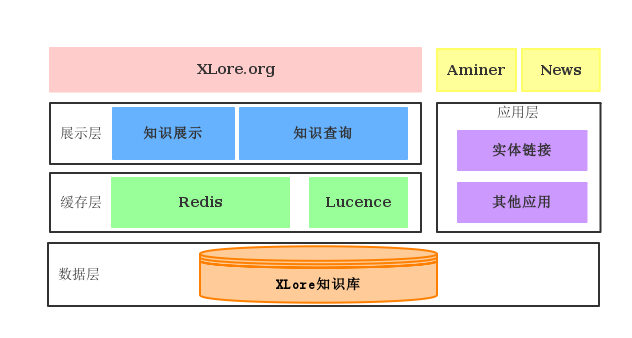
\includegraphics[width=0.9\columnwidth]{xlore-architecture}
  \caption{XLore系统架构图}
  \label{fig:xlore-architecture}
\end{figure}

为了语义化信息,我们将数据依托于图数据库。当前知名的的图数据库有Neo4J\footnote{http://neo4j.com/},AllegroGraph\footnote{http://allegrograph.com/allegrograph/},Virtuoso\footnote{http://virtuoso.openlinksw.com/}等,鉴于我们的数据是以三元组的形式组织的,更适用于triple-store类型的数据库,因此我们选用商业版Virtuoso(Virtuoso Universal Server)作为存储容器。

Virtuoso是由OpenLink软件公司开发的一个混合型数据库,它既支持传统的RDBMS数据,也支持RDF等其他图类型数据的存储与查询。其商业版本(Virtuoso Universal Server)可支持多CPU处理、多会话访问以及集群网络环境等。商业版Virtuoso是闭源的,但OpenLink公司提供一个名为OpenLink Virtuoso的开源版本[GitHub链接],供使用者编译与尝试。

为了提高搜索效率,我们使用Redis\footnote{http://redis.io/}充当缓存。为了给出更好的搜索体验,用为各个元素标签及其URI建立了索引,使用Lucence的模糊查询代替完全匹配,返回更多相关搜索结果。

Web框架采用JSP+Struts2.0搭建,运行在Tomcat7.0 Web服务器上。页面设计基于当前最受欢迎的Bootstrap前端框架。

对于概念与实例,我们基于D3.js可视化库\footnote{https://d3js.org/},提供了关系可视化,包括概念-子概念的关系,实例-相关实例的关系。

\subsection{XLore知识展示}
图\ref{fig:xlore-home}为XLore网站首页。截止到2015年8月,我们的跨语言知识库中包含有663,740个概念、56,449个属性、10,856,042个实例。首页以表格的形式提供了顶层及其下两层的概念层及其统计数据,点击左边“+”按钮可获得子概念样例。除此之外,首页列出了一些实例例子,点击可直接查看相应实例页面。

\begin{figure}[H] 
  \centering
  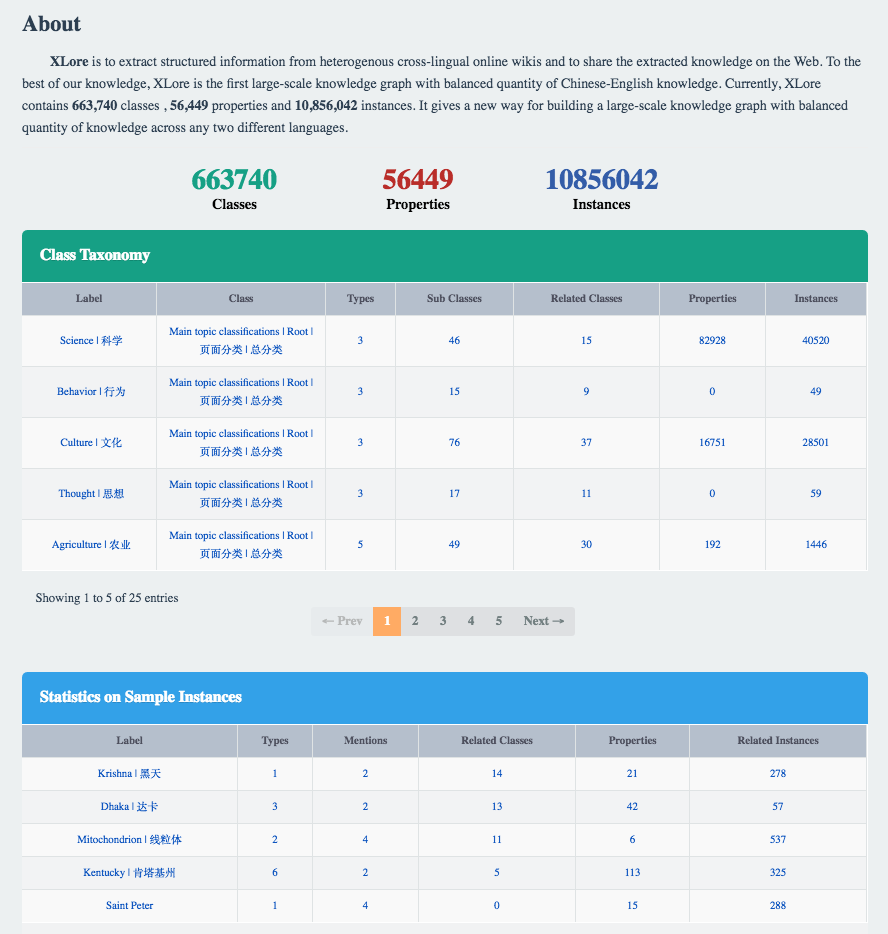
\includegraphics[width=0.8\columnwidth]{xlore-home}
  \caption{XLore网页系统首页}
  \label{fig:xlore-home}
\end{figure}

作为双语知识库,XLore提供了语言切换功能,同时满足中文用户与外文用户的用户体验。

XLore网站为三种知识提供展示,分别为概念、属性、实例。
概念页面以绿色为主色调,显示了概念中英文标签、父概念、子概念、相关实例等信息。
属性页面使用紫色色调,展示了中英文标签、属性类型(DateType与ObjectType)、相关实例、定义域(Domain)与值域(Range)等。 
实例页面色调为蓝色,展示了中英文标签、实例图像、所属概念、摘要、信息框(包括中英文信息),URL多种信息。三种页面中,涉及到的双语内容,我们以\textit{中文[英文]}的格式展示每条信息,如果网站语言为英文,则将英文展示在前,格式变为\textit{英文[中文]}。当涉及到四个百科内容且无法融合,我们利用网页标签分栏的形式分别展示不同百科信息,如图\ref{fig:xlore-page}。

\begin{figure}[H] 
  \centering
  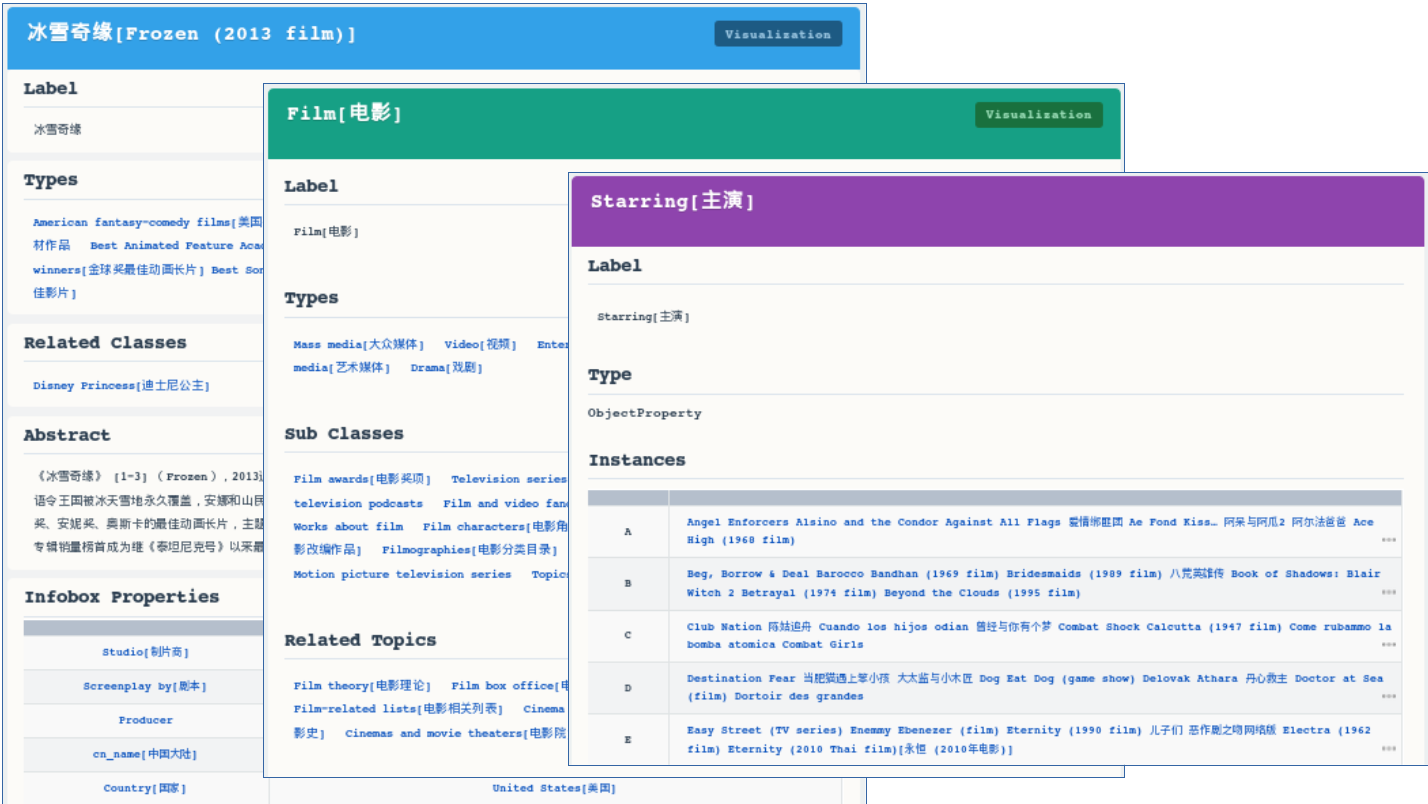
\includegraphics[width=1\columnwidth]{xlore-page}
  \caption{XLore实例、概念、属性页面展示}
  \label{fig:xlore-page}
\end{figure}

\subsection{XLore关系可视化}

XLore提供了两个数据可视化展示,分别为概念上下位关系可视化与相关实例可视化,图\ref{fig:xlore-visualization}为可视化例子,图\ref{fig:xlore-visualization-instance}显示指定实例及其相关实例,以相关领域划分,直接相关实例(信息框中实例)距离近,间接相关实例(文本内链接实例)距离较远;图\ref{fig:xlore-visualization-concept}显示指定概念及其子概念(黄色)、父概念(绿色)。

\begin{figure}[H] 
  \centering
  \begin{subfigure}{7.2cm}
    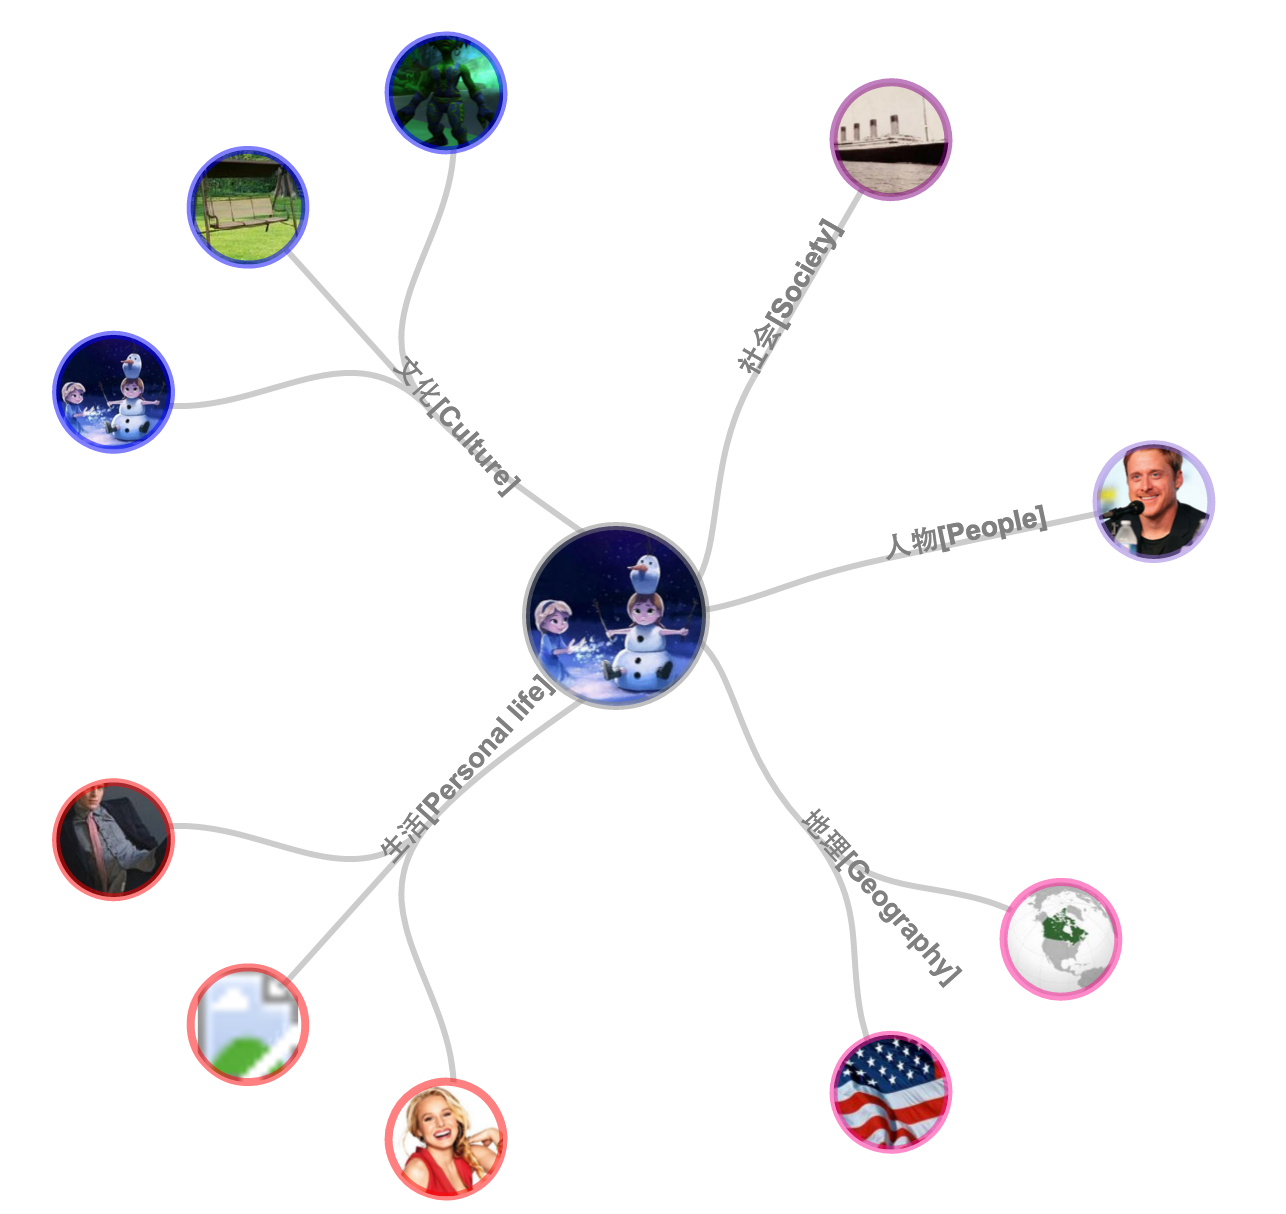
\includegraphics[height=5.4cm]{xlore-visualization-instance}
    \caption{实例可视化例子(阿甘正传)}
  \label{fig:xlore-visualization-instance}
  \end{subfigure}
  \hspace{0.01cm}%
  \begin{subfigure}{7.2cm}
    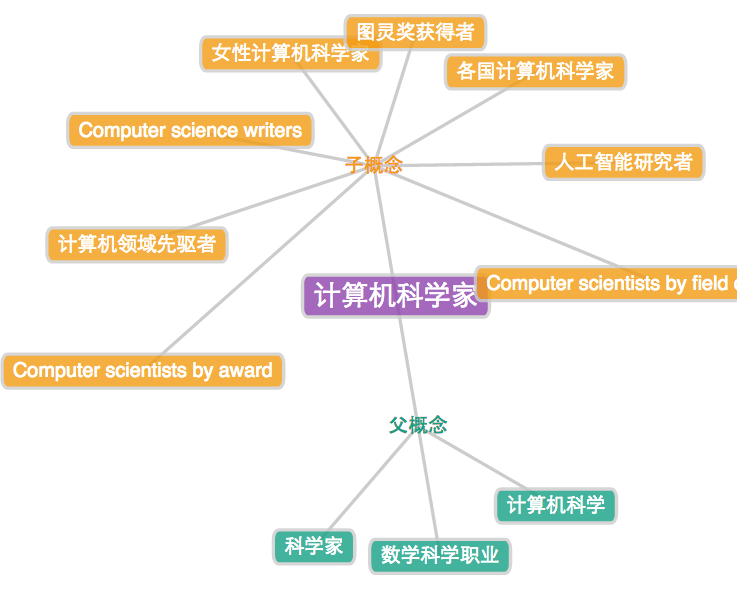
\includegraphics[height=5.4cm]{xlore-visualization-concept}
    \caption{概念可视化例子(计算机科学家)}
  \label{fig:xlore-visualization-concept}
  \end{subfigure}
  \caption{关系可视化例子}
  \label{fig:xlore-visualization}
\end{figure}

%\begin{figure}
%\centering
%\begin{subfigure}{7.2cm}
%\centering
%\includegraphics[height=5.4cm]{s2c-pie}
%\caption{饼状图}
%\label{fig:pie}
%\end{subfigure}
%\hspace{0.01cm}
%\begin{subfigure}{7.2cm}
%\centering
%\includegraphics[height=5.4cm]{s2c-scatter}
%\caption{散列图}
%\label{fig:scatter}
%\end{subfigure}
%\caption{新闻句子与对齐用户评论数分布图}
%\label{fig:s2c}
%\end{figure}

\subsection{XLore知识查询}
XLore提供搜索框文本查询与SPARQL语句查询两种查询方法。

搜索框显示于每个页面的上方,输入要查询的中文或英文字符串,点击“搜索”或按Enter键,即获得模糊查询结果。用户可根据需求选择搜索概念还是实例,或者属性,默认情况下,系统会同时返回三类搜素结果,用户可通过切换标签查看。图\ref{fig:xlore-search-engine}为搜索结果页面展示。

\begin{figure}[H] 
  \centering
  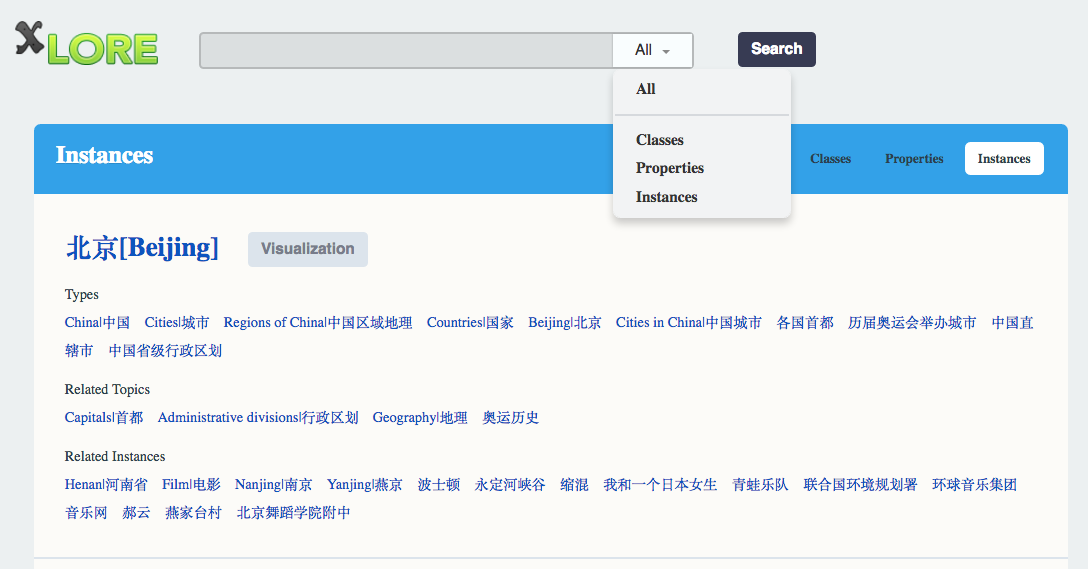
\includegraphics[width=0.9\columnwidth]{xlore-search-engine}
  \caption{XLore文本搜索框与搜索结果展示}
  \label{fig:xlore-search-engine}
\end{figure}

另一方面,对于专业人士,我们提供SPARQL查询页面,如图\ref{fig:xlore-sparql-endpoint}所示,输入正确的sparql语句,返回结果中可看到我们对知识库schema的定义。另外,为了防止sql注入造成的攻击与数据库崩溃,我们采取了xxx的安全措施。

\begin{figure}[H] 
  \centering
  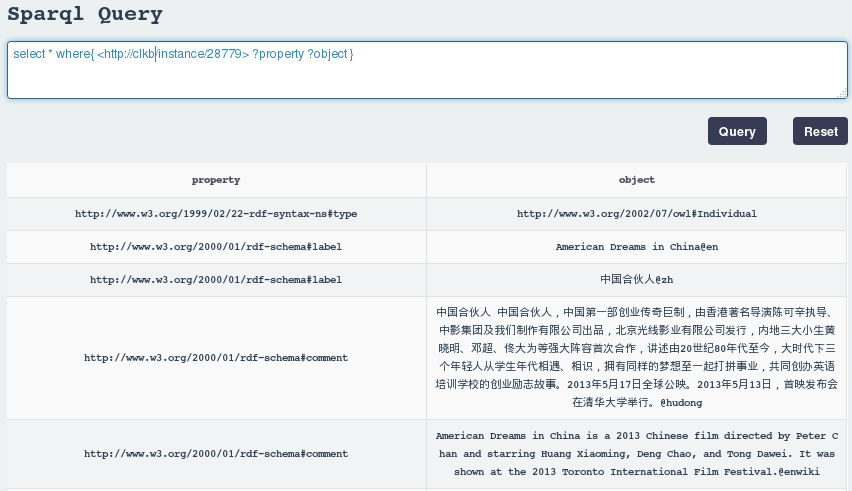
\includegraphics[width=0.9\columnwidth]{xlore-sparql-endpoint}
  \caption{XLore SPARQL 搜索框与搜索结果展示}
  \label{fig:xlore-sparql-endpoint}
\end{figure}

\section{XLore实体链接接口}
\label{sec5:entity-linking-api}

知识库中的实例与概念表征着世界上唯一一个实体,知识库还存有实体的信息、实体间的关系等等,因此知识库在实体相关研究中起着举足轻重的作用,实体查询、实体链接、实体推荐等应用多基于构建完备的知识库。

对同一个实体,外界有不同的称呼,比如演员刘德华,有昵称华仔、Andy。另一方面,一个名称可能表征不同实体,比如SVM在机器学习领域是\textit{Support Vector Machine}的缩写,但在新闻报道中可能是\textit{Stored Value Marketing公司}的简称。给出一个名称,在知识库中找出其对应的真正实体,被称作{\heiti 实体链接}任务。如果我们能成功抽取出文本中的实体名称,并准确匹配出名称所代表的实体,对于该文本的理解有很大意义。

XLore作为一个通用领域的跨语言知识库,在囊括了大量知识的基础上,提供了基于实体-名称词典扩展的实体链接接口。

XLore实体链接接口提供了四种类型的查询:
\begin{enumerate}[1.]
\item 通用领域的名称查询:给出一个通用领域的名称,返回其在XLore中最可能指向的一个或几个实体以及实体的中英文信息;
\item 通用领域的文本实体查询:给出一串文本,对文本进行实体名称抽取后,返回名称列表中各名称在XLore中最可能指向的实体及实体的中英文信息;
\item 学术领域的名称查询:给出一个学术领域的名称,如“机器学习”,返回其在XLore中学术领域指向的实体以及实体的中英文信息。
\item 学术领域的文本查询:给出一个学术领域相关的文本,经过术语抽取后,返回术语在XLore中学术领域指向的实体以及实体的中英文信息。
\end{enumerate}

该接口框架如图\ref{fig:entity-linking-architecture}
该接口以中英文名称或文本为输入,经过实体抽取、实体候选生成、实体排歧,确定与名称和上下文最匹配的实体,返回实体列表与中英文实体信息。
\begin{figure}[H] 
  \centering
  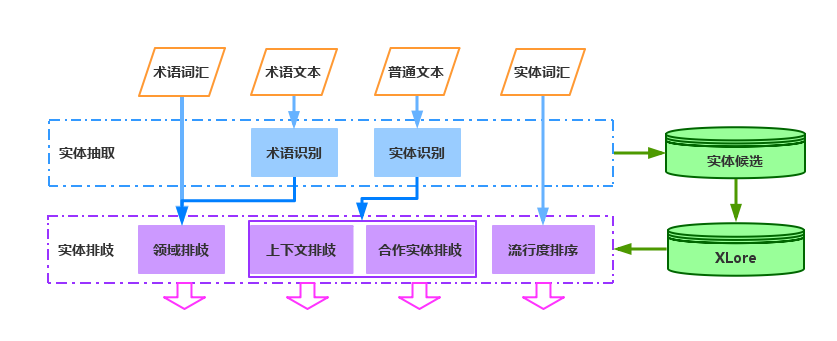
\includegraphics[width=1\columnwidth]{entity-linking-architecture}
  \caption{XLore 实体链接接口框架图}
  \label{fig:entity-linking-architecture}
\end{figure}

\subsection{实体抽取}
对于给定的长文本,首先要提取出其中可以分析的实体文本。该阶段,我们引入成熟的实体或术语抽取工具,包括:
\begin{itemize}
\item 通用领域实体抽取,中文使用开源中文分词工具jieba\footnote{https://github.com/fxsjy/jieba},主要获得其中nt、nz、nr、ns类型的实体;英文使用Stanford Parser\footnote{http://nlp.stanford.edu/software/lex-parser.shtml}解析工具,获取PERSON、LOCATION、ORGANIZATION三类实体。
\item 学术领域实体抽取使用来自微软的学术术语抽取工具。
\end{itemize}

\subsection{实体候选生成}

实体候选从名称-实体词典中,通过名称获取相应的所有实体。其中,中英文名称-实体词典从中英文维基百科、百度百科、互动百科中抽取,选取以下几种元素构成:

\begin{enumerate}[1.]
\item 各百科的词条标题:百科中的每个词条都描述唯一实体,并维护着这个实体的相关信息。一般来说,词条标题是该实体公认的、最普遍的名称。对于无歧义的标题,记录其完整标题即可。然而,有些标题有多种含义。在百科中,如果一个标题有歧义,百科会通过在标题后加入分类信息来实现消歧,比如百度百科中,苹果(蔷薇科苹果属果实)代表一种水果,苹果(苹果产品公司)代表美国一家高科技公司,这种情况,标题“苹果”为实体“苹果(蔷薇科苹果属果实)”(在XLore中有对应ID)的一个名称。
\item 各百科的文本内链接:百科词条的文本中,经常会有一些实体名称,以超链接的形式存在,指向该实体对应的词条。这个超链接的锚文本,可以看作是指向实体的同义词或别称,锚文本与实体词条构成一条名称-实体信息。
\item 各百科的消歧页面:如果一个名称可能对应多个实体,百科会为其创建一个歧义页面,供用户按所需选择词条。比如,“苹果”是一个歧义词汇,则歧义页面中会列举“苹果(蔷薇科苹果属果实)”、“苹果产品公司”等词条。维基百科通过“苹果\_(消歧义)”这样的页面[链接地址]展示词条,百度百科则通过为“苹果”父词条[链接地址]创建subview子词条来进行区分,如果一个词条没有歧义,则它的网页地址以id定位;如果一个词条有多种意思,则它的id页面为歧义页面,各子词条网址用subview id定位。消歧页面对于抽取实体的别称也有很大贡献。
\item 维基百科的重定向页面: 维基百科通过不断进行词条整理与更新,对一些陈旧的、非标准词条,或公认的缩写名称、别称等,将其自动定位到同一实体的标准词条页面上。原来的旧名称、缩写等可以看作实体的名称。比如中文维基中,“Microsoft”会被重定向到“微软”页面。
\end{enumerate}

以2016年3月的中英文维基百科、2014年12月的百度百科、互动百科为数据源,我们获得名称-实体关系数量如表 \ref{tab:mention-entity}所示:

\begin{table}[htb]
  \centering
  \caption 名称-实体关系对抽取数量统计
  \label{tab:mention-entity}
  \begin{minipage}[t]{0.8\textwidth} 
    \begin{tabularx}{\linewidth}{lXXXX}
      \toprule[1.5pt]
      {\heiti 类型} & {\heiti 英文维基} & {\heiti 中文维基} & {\heiti 百度百科} & {\heiti 互动百科} \\\midrule[1pt]
      标题 & 16.345,549 & 2,739,609 & 1 & 1 \\
      内链接 & 45,650,452 & 6,784,030 & 1 & 1 \\
      消歧页面 & 1 & 2550 & 174,862 & 24,158 \\
      重定向页面 & 2,759,377 & 362,767 & -  & - \\
      合并总对数 & 1 & 1 & 1 & 1 \\
      \bottomrule[1.5pt]
    \end{tabularx}
  \end{minipage}
\end{table}

抽取结果合并后,获得中英文名称-实体对应关系总数量为67,429,935对。我们只保留在XLore中能命中的实体,最终获得{\heiti 23,635,510}对关系。平均每个实体有1.97个名称,每个名称可能对应1.32个实体。
%17845907个mention, 11987986个entity

在抽取过程中,我们对名称-实体的出现频数进行了记录,用于之后的排歧工作。以\textit{名称 \ 实体知识库uri \ 出现频数}为格式存储数据,并以名称为索引,将数据导入到MySQL数据库中,便于查询。

\subsection{实体消歧方法}
实体消歧主要是对候选实体的匹配可能性进行排序,
对于通用领域的名称查询,因为没有任何上下文信息,我们只能直接以流行度(出现频数)从高到低排序,返回受到广泛认可的一个或多个实体信息。
对于学术领域的查询,我们利用知识库特有的分类体系,凭借领域约束,将实体的查找限制在相关概念下。

对于通用领域的文本查询,我们根据上下文,为每个名称返回最相关的实体。具体来说,对于给定名称,为其每个候选实体计算一个背景相关度,最相关的最可能为所求实体。
给定一段文本$T$,经过实体抽取后获得实体名称集合$M$,对于$m_i \in M$,计算$m_i$的一个实体候选$c_{i,j} \in C(m_i)$的相关度:
\begin{itemize}
\item 1.  计算上下文相关度($R_a$):认为自身信息与上下文有关的实体更相关,提取名称文本$T$,与实体的摘要$A(c_{i,j})$进行Cosine相似度计算。

\item 2.  计算合作实体相关度($R_e$):认为与文中其他实体有语义关系的实体更相关,提取根据文中其他名称$M'=$对应的实体候选$C(M') = $,与本名称的实体候选的相关实体,即文本中的链接实体$I(c_{i,j})$做交集。
\begin{equation}
{ R }_{ e }=\frac { \left| C\left( M' \right) \cap I\left( { c }_{ i,j } \right)  \right|  }{ \left| I\left( { c }_{ i,j } \right)  \right| +1 } 
\end{equation}

\item 3.  取两个相关度的最大值。
\begin{equation}
R = \max{ \left(R_a, R_e \right)}
\end{equation}
\end{itemize}
$R_{i,j}$ 即为实体候选$c_{i,j}$与名称$m_i$的相关度,$R_{i,j}$越大,$c_{i,j}$越可能是所求实体。

\subsection{实体链接接口的应用}
该实体链接接口的学术领域名称查找功能,应用在Aminer学术搜索系统\footnote{https://aminer.org/}的学术知识展示模块上,如图\ref{fig:el-aminer}所示:用户在搜索学术领域词汇时,右边会显示该词汇对应的学术实体信息,及其相关上下文概念。
\begin{figure}[H] 
  \centering
  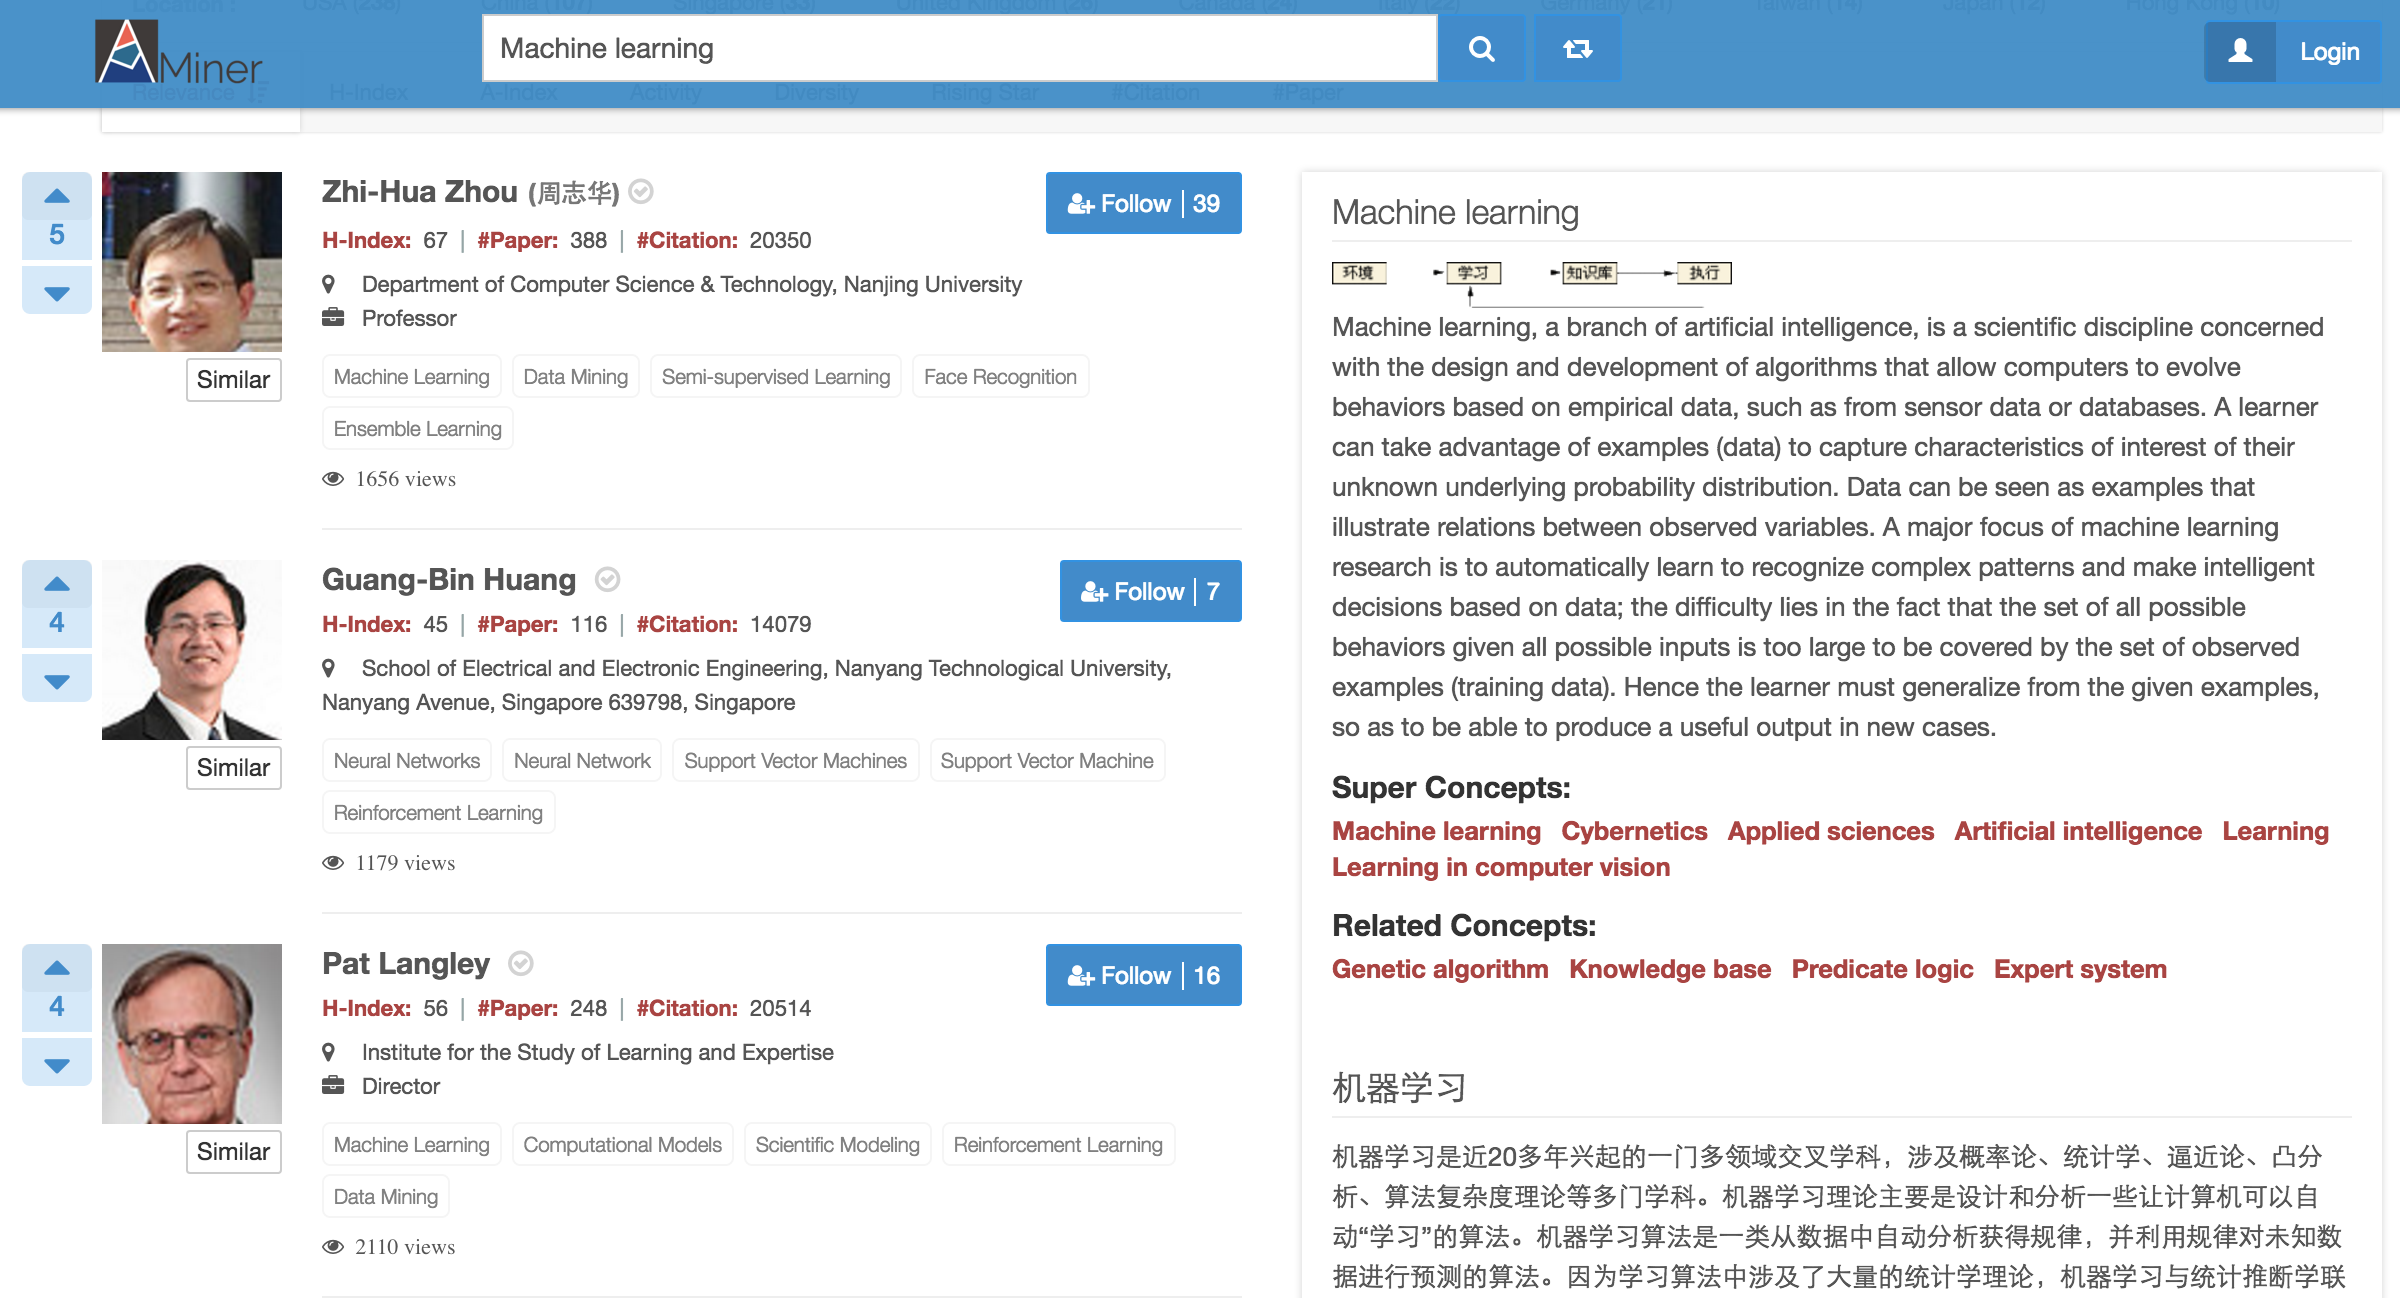
\includegraphics[width=0.8\columnwidth]{el-aminer}
  \caption{XLore实体链接接口在Aminer上的应用}
  \label{fig:el-aminer}
\end{figure}

通用领域名称查找功能,应用在新闻分析系统NewsMiner\footnote{http://newsminer.net}上,分析新闻文本,提供实体信息。如图\ref{fig:el-newsminer}所示:
\begin{figure}[H] 
  \centering
  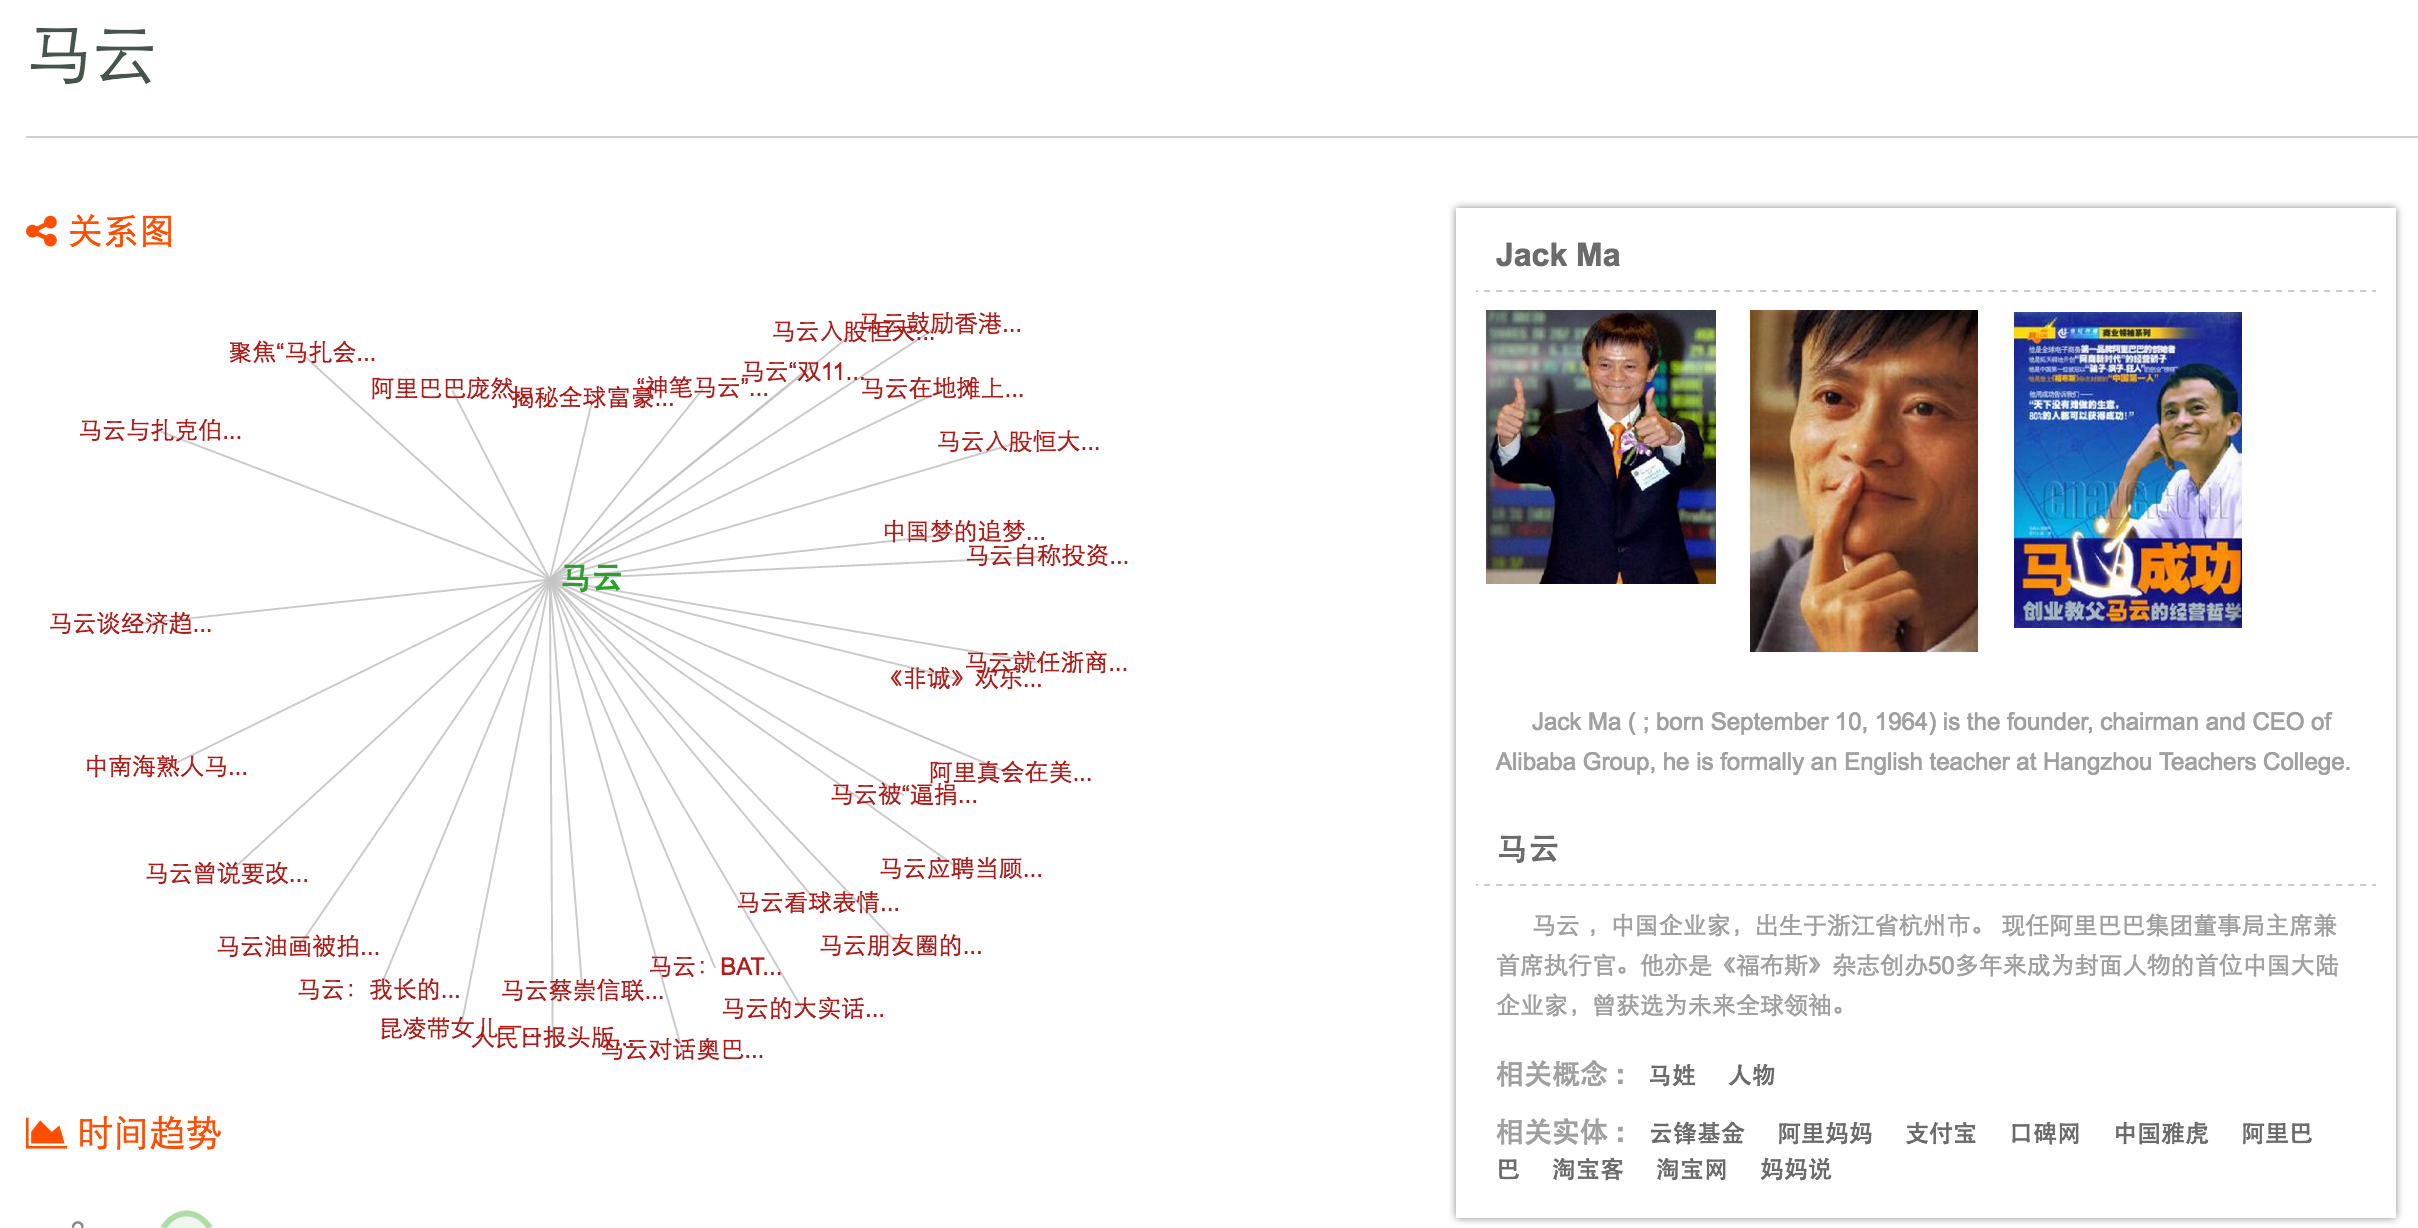
\includegraphics[width=0.8\columnwidth]{el-newsminer}
  \caption{XLore实体链接接口在NewsMiner上的应用}
  \label{fig:el-newsminer}
\end{figure}

\section{本章小结}
本章节介绍一个从多个在线百科中抽取数据,构成跨语言知识库的方法。我们从网页中抽取结构化数据并统一数据格式,生成并扩展跨语言链接信息来融合双语知识。最终获得的知识库XLore,包含663,740个概念,56,449个属性以及10,856,042个实例。

此外对XLore系统进行了详尽的介绍:为了进一步了解数据情况,我们搭建了网站展示XLore知识,将数据直观地展现出来。同时,为了提高知识库的可用性,开发了实体链接接口,提供通用领域与指定领域的语义信息,也为下一步更精确的实体链接工作,做好铺垫。

